\documentclass[10pt]{beamer}

\usepackage[utf8]{inputenc}
\usepackage{tcolorbox}
\usepackage{tikz}
\usepackage{tikz-3dplot}
\usetikzlibrary{intersections,calc,,angles,quotes,through}
\usepackage{amsmath}
\usepackage{graphicx}
\usepackage{cases}
\def \heart {\textcolor{blue}{$\heartsuit$} }
\def \C {\mathcal{C}}
\def \orthog {\underline{\perp}}
\def\arcos{\operatorname{arcos}}
\def \deg {^{\circ}}

\newcommand{\vect}[1] {
  \overrightarrow{#1}}

\tcbset{%
	basic/.style={colframe=black,
		      colback=white,
		      top= 0mm,
		      bottom = 2mm,
		      boxsep=0mm
		      }
}
\tikzset{
    invisible/.style={opacity=0},
    visible on/.style={alt={#1{}{invisible}}},
    alt/.code args={<#1>#2#3}{%
      \alt<#1>{\pgfkeysalso{#2}}{\pgfkeysalso{#3}} % \pgfkeysalso doesn't change the path
    },
  }

    
\begin{document}  
    \beamertemplatenavigationsymbolsempty
    \setlength{\abovedisplayskip}{0pt}
    \setlength{\belowdisplayskip}{0pt}
    \frame{
	  
	  \frametitle{Q2 Juillet 2002.}
	  %\renewcommand{\theenumi}{\alph{enumi})}
	  Dans le plan muni d’un repère orthonormé $Oxy$, on note $\mathcal{P}$ la parabole d’équation
	  $y = x^2$ et $P$ le point de $P$ d’abcisse $1$. Quel est le lieu des sommets des paraboles
	  d’axe parallèle à $Oy$ et orthogonales à $\mathcal{P}$ en $P$ (dire que deux paraboles sont
	  orthogonales en $P$ signifie qu’elles passent par $P$ et que leurs tangentes en $P$ sont
	  perpendiculaires).
	  \vfill
	  
	  \pause
	  
	   \begin{tcolorbox}[basic] \smallskip
	      \begin{columns}[t]
		 
		 \column{.5\textwidth}\centering
		      
		      \underline{Hypothèses}\ \smallskip 
		      	      
		      \hspace{-14mm}$\mathcal{P} \equiv y=x^2,$  \\ \smallskip
		      $\mathcal{P_L} \equiv$ $\begin{cases}
                      \text{Axe vertical}, \\
		      \mathcal{P_L}(P) \bot  \mathcal{P}(P), \\
		      \ni P.
		       \end{cases}$
		      
		  
		  \column{.5\textwidth}\centering
		      
		      \underline{Inconnues} \\
		      \smallskip
		      Equation des sommets de $\mathcal{P_L}$.
		
	      \end{columns}
	  \end{tcolorbox}
    }

    \frame{ 
	  % résolution ex1

		\begin{columns}[t]\onslide<+->
				  \column{.5\textwidth}\centering 
		

			          \underline{Dessin}\\
			
				  \begin{figure}[h]
				  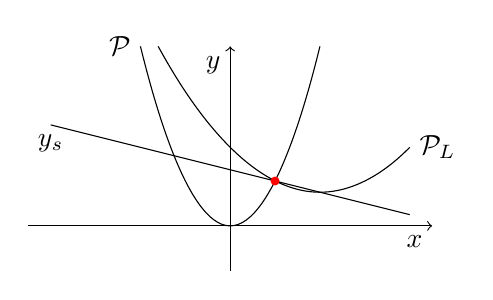
\begin{tikzpicture}[scale=0.57]
					%\draw[help lines] (-3,-3) grid (3,3); 				
					%AXES
					\draw[->] (0,-1) -- (0,4) coordinate[label=below left:$y$]();
					\draw[->] (-4.5,0) -- (4.5,0) coordinate[label=below left:$x$]();
					%P_1 et P_2
					\draw (-2,4) coordinate[label=left:$\mathcal{P}$]() parabola bend(0,0) (2,4);
					\draw (-1.605,4) parabola bend(2,0.75) (4,1.75) coordinate[label=right:$\mathcal{P}_L$]();
					\draw[visible on=<2>] (-4,2.25) node[below]{$y_s$} -- (4,0.25);
					\fill[visible on=<2>,red] (1,1) circle (0.1);
					
				  \end{tikzpicture}
				  \end{figure}
			
				  \begin{tcolorbox}[basic] 
				      
				    \smallskip
				    \underline{Hypothèses}\smallskip 
				    
				    \hspace{+7mm}$\mathcal{P} \equiv y=x^2,$  \\
				    \begin{numcases}{\mathcal{P_L} \equiv}
				    \text{Axe vertical}, \\				    
				    \mathcal{P_L}(P) \bot  \mathcal{P}(P), \\
				    \ni P.
				    \end{numcases}
							      
				    \underline{Inconnues} \\
				    \smallskip
				    Equation des sommets de $\mathcal{P_L}$. 
				    \end{tcolorbox}
		
		
		\column{.5\textwidth}\centering
		
		\underline{Résolution}\\ \flushleft
		\begin{enumerate}
		 \item $\mathcal{P_L} \equiv y = a(x-x_s)^2 + y_s$. \\ \smallskip
		       $\hspace{3cm}(a\neq 0)$
		\end{enumerate} \bigskip
		
		$P=(1,1)$. \medskip
		
		\heart Deux droites sont $\bot$ si le produit de leur coefficient angulaire vaut $-1$. \\ \medskip
		
		\begin{itemize}
		 \item[2.] $\mathcal{P_L}'(1)\mathcal{P}'(1) = -1$.
		\end{itemize}
		$\rightarrow \qquad 4\ a(1-x_s)=-1 \qquad \hspace{2mm} (\dag)$. \\ \bigskip
		
		
		
		\begin{enumerate}
		 \item[3.] $\mathcal{P_L}(1) = 1$.		   
		\end{enumerate}
		$\rightarrow \qquad a(1-x_s)^2 + y_s = 1 \qquad (\ddag)$. \\ \bigskip
		
		$(\dag)\ a = \dfrac{1}{4(x_s-1)}. \quad (x_s \neq 1)$ \\ \medskip
		\onslide<+->$(\ddag)\ y_s = -\dfrac{x_s}{4} + \dfrac{5}{4}. \quad (x_s \neq 1)$\hfill $\qed$
		
		
		\medskip
		
		 
	
		
		
		\hfill $\qed$
   
	   \end{columns}
	
    }
	  
  
\end{document}
